%%
%% Ocelotl User Guide
%%

\documentclass[twoside]{article}
\usepackage[a4paper]{geometry}
\usepackage[utf8]{inputenc}
%\usepackage[T1]{fontenc}
\usepackage{RR}
\usepackage[hidelinks]{hyperref}
\usepackage{epsfig}
%\usepackage[english]{babel}
\usepackage{cite}
\usepackage{float}
\usepackage{graphicx}
\usepackage{subcaption}
\usepackage{textcomp}
\usepackage{wrapfig}

\usepackage{listings}
%%
%% date
\RRdate{January 2015}
%%
%%
\RRauthor{
Youenn Corre \thanks{INRIA, youenn.corre@inria.fr} \\
Damien Dosimont \thanks{INRIA, damien.dosimont@imag.fr} 
}

%% On each even page
\authorhead{Ocelotl User Guide}
%% French title
\RRtitle{Ocelotl User Guide}
%% English title
\RRetitle{Ocelotl User Guide}
%%
\titlehead{Ocelotl User Guide}
%%
\RRprojet{MOAIS}
%%
\URRhoneAlpes 
%%
\RCGrenoble 
%%
\abstract{This guide describes the Ocelotl tool, in its version 1.1.3, available at the following github repository: \url{https://github.com/soctrace-inria/ocelotl}.}

%%=====================================================================
%%=====================================================================
\begin{document}

\begin{sloppypar} %% avoid long words exceeding margins
%%=====================================================================
%%=====================================================================

%\shorthandoff{:} %% Remove the space before the colon
\interfootnotelinepenalty=10000 %% allow long footnotes

%%=====================================================================
%% Custom commands
\newcommand{\parag}[1]{\paragraph{#1}\mbox{}\\}
\newcommand{\subparag}[1]{\subparagraph{#1}\mbox{}\\}
\newcommand{\subsubparag}[1]{\subparagraph{#1}}
%% 
%% Itemize
\renewcommand{\labelitemi}{$\bullet$}
\renewcommand{\labelitemii}{$\circ$}
%%=====================================================================

%%
\makeRT 
%%

%%=====================================================================
\renewcommand{\contentsname}{Table of contents}
\tableofcontents
\newpage
%%=====================================================================
%=====================================================================
\section{Introduction}
\label{intro}

%=====================================================================

Ocelotl is a tool to explore, analyze and visualize execution traces through aggregation techniques. It is part of the SoC-Trace project, and as such, it is integrated in the Framesoc framework as an Eclipse plug-in. 

\section{Installation}
Please refer to the installation procedure described on the Ocelotl wiki page: \url{https://github.com/soctrace-inria/ocelotl/wiki/User-Guide}.

\section{Launch Ocelotl}

\begin{figure}[h!]
	\centering
    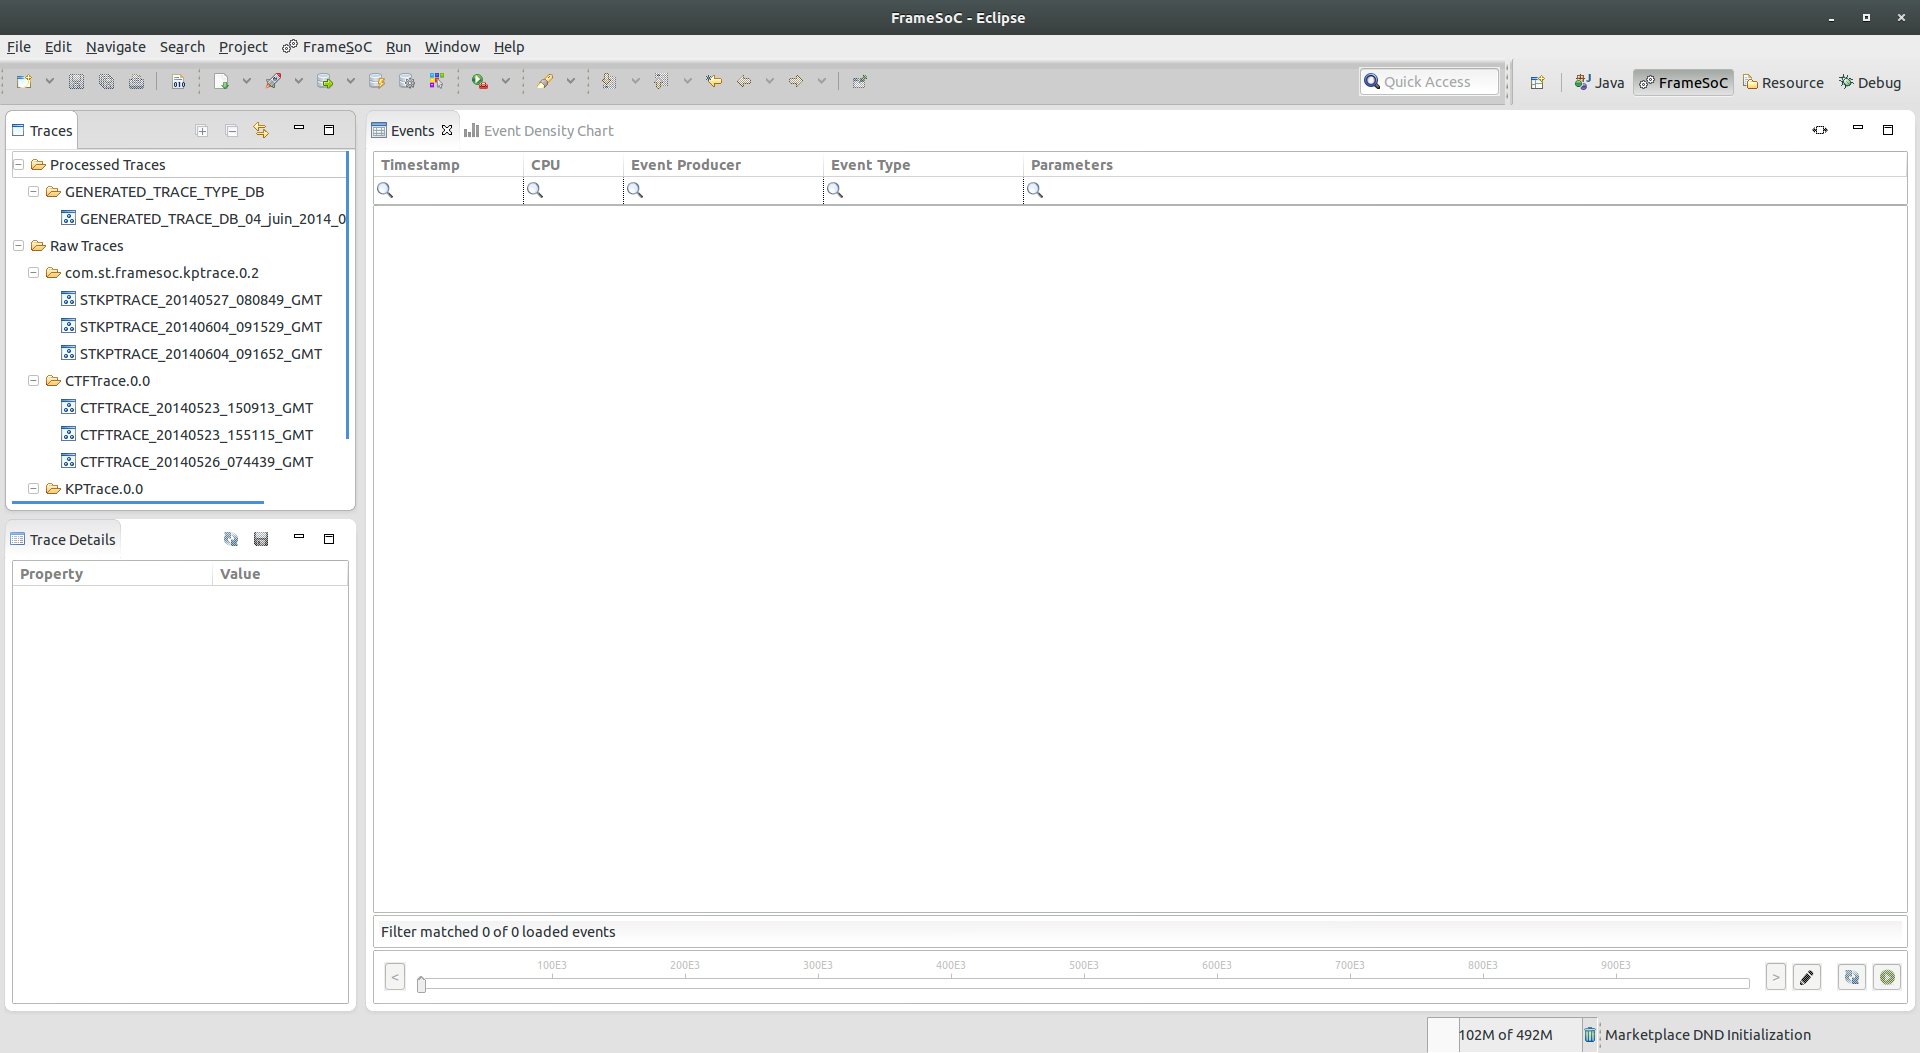
\includegraphics[width=1.0\textwidth]{images/framesoc_launch.png}
	\caption{Framesoc Eclipse Workbench at startup}
	\label{frameLaunch}
\end{figure}

In order to launch Ocelotl:

\begin{enumerate}
	\item 
	\begin{itemize}
		\item Go to the Framesoc menu, choose the \textit{Trace Analysis} entry and click on \textit{Launch Analysis Tool}. 
		\item Or click on the \textit{Analyze Trace} icon.
	\end{itemize}

	\begin{figure}[h!]
		\centering
		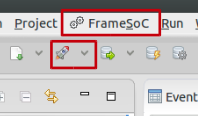
\includegraphics[scale=0.5]{images/labeled.png}
		\caption{The Framesoc menu and the \textit{Analyze Trace} icon}
		\label{launchOcelotl}
	\end{figure}
	
	\item Select the Ocelotl tool.
	\begin{figure}[h!]
		\centering
		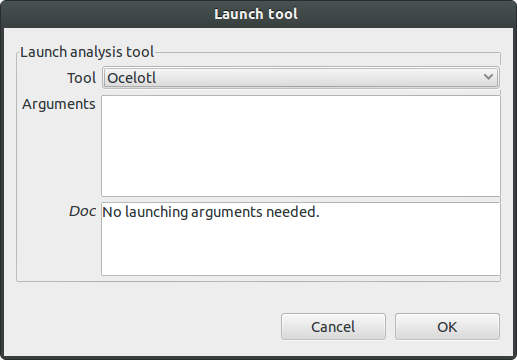
\includegraphics[scale=0.5]{images/launch_tool.png}
		\caption{Ocelotl launching window}
	\end{figure}
	\item No argument is needed so just click \textit{OK}.
\end{enumerate}

The Ocelotl tool view should open, as illustrated in Fig. \ref{ocelotlOverview}.
\begin{figure}[h!]
	\centering
	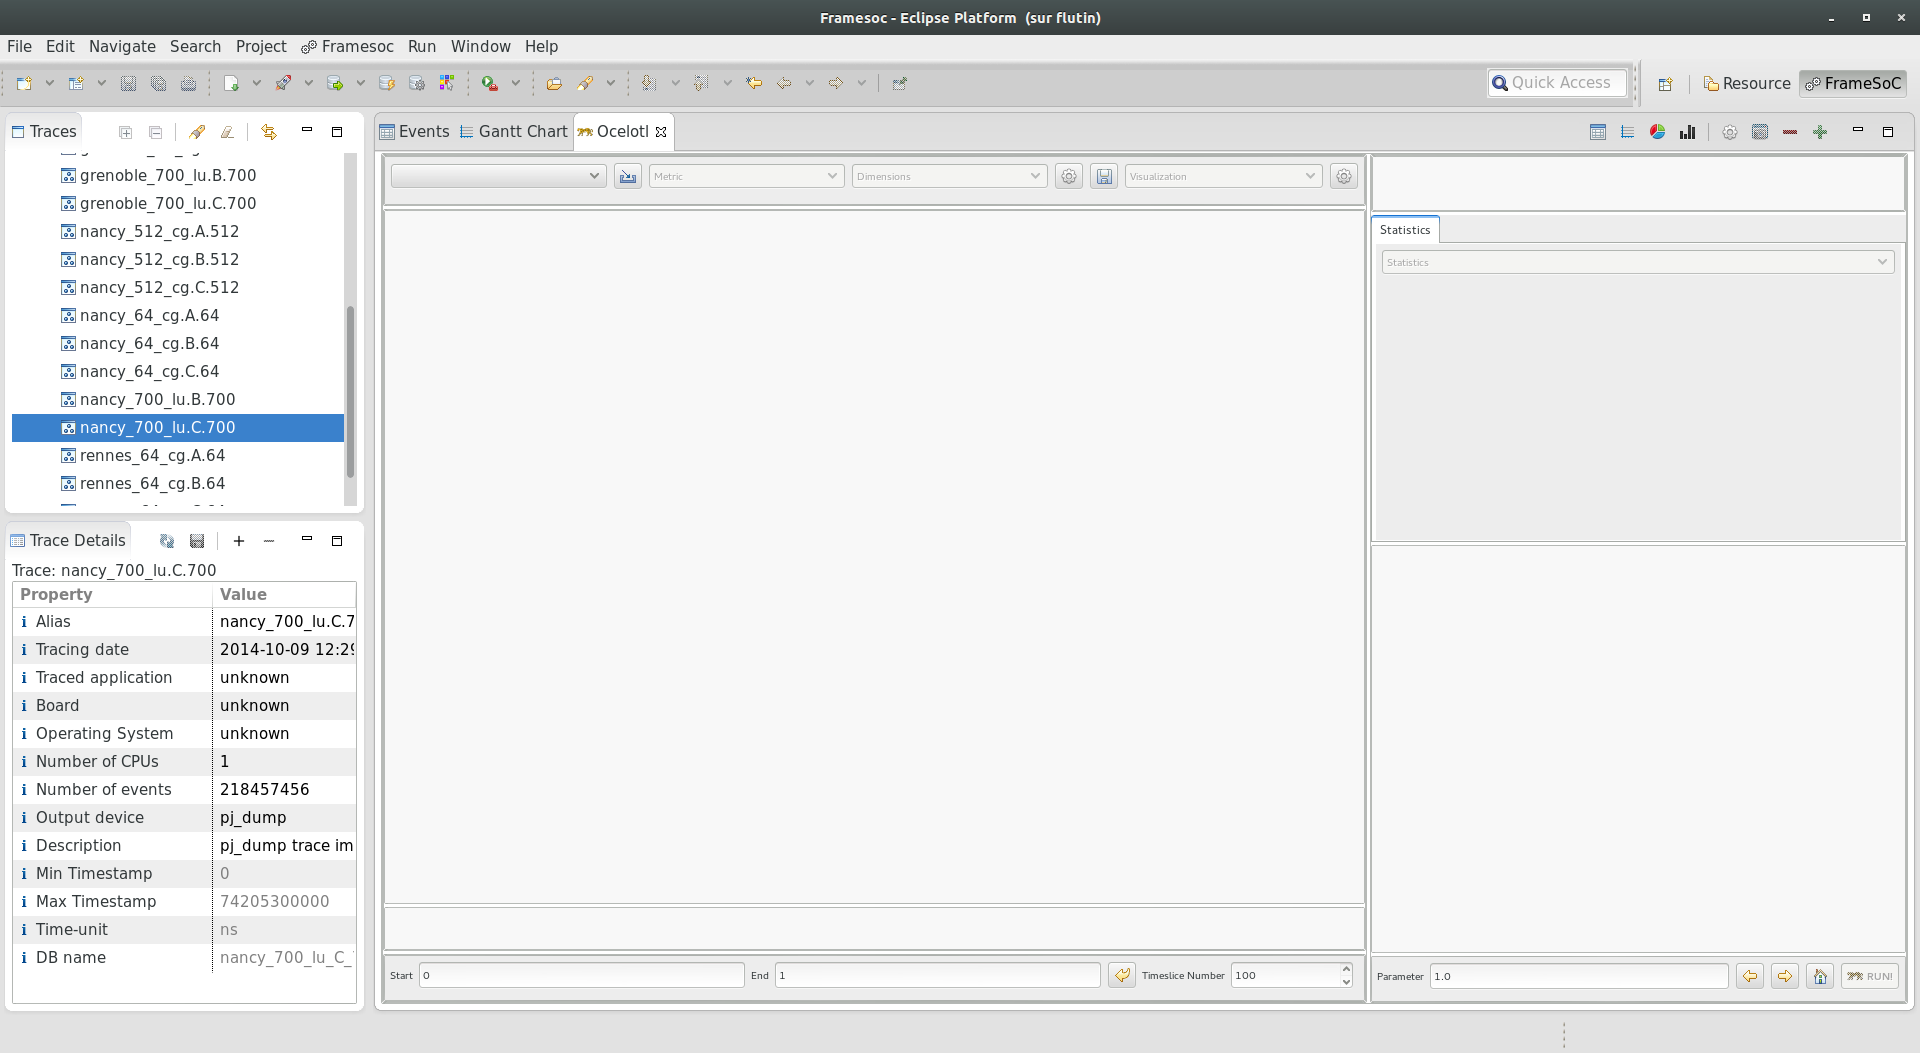
\includegraphics[width=1.0\textwidth]{images/ocelotl_startup.png}
	\caption{Ocelotl at startup}
	\label{ocelotlOverview}
\end{figure}


\section{Ocelotl Features}
In this section, we describe how to load a trace, launch the analysis and explore the results by modifying parameters. 

\subsection{Load a Trace}
\begin{figure}[h!]
	\centering
	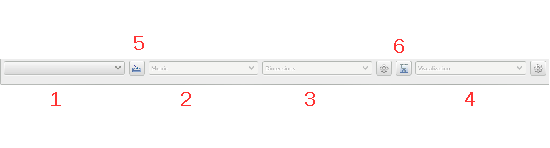
\includegraphics[width=\textwidth]{images/traceSelection_labeled.pdf}
	\caption{Trace configuration interface}
	\label{traceConf}
\end{figure}

\subsubsection{Select a Trace}

At the top of the Ocelotl window, the \textit{Trace Overview} tool bar allows to select a trace to analyze (element \textcolor{red}{1} in Fig. \ref{traceConf}). It shows the traces already exported in Framesoc. Once a trace is selected, the default settings compatible with the trace are automatically selected. However it is possible to change these settings, as described in the following subsections. 

It is also possible to load a trace from the Framesoc Trace tree (the frame on the top left in Fig. \ref{frameLaunch}): right-click on the trace that should be load and select \textit{Show in Ocelotl} in the context menu. By using that way to load a trace, it is possible to launch multiple instances of Ocelotl, up to five simultaneous instances maximum\footnote{This limit can be set in the Framesoc configuration file. Please refer to the Framesoc user doc to configure Framesoc (\url{https://github.com/soctrace-inria/framesoc/blob/master/src/fr.inria.soctrace.maven.repository/archive/doc/framesoc_user_guide.pdf?raw=true}).}.

\subsubsection{Metric Selection}
The \textit{Metric} combo (element \textcolor{red}{2} in Fig. \ref{traceConf}) displays the metrics compatible with the current trace.
At the moment, the available metrics are: 
\begin{itemize}
	\item \textit{Events} which performs an analysis based on the event occurrences. This type of analysis is compatible with all the traces.
	\item \textit{States} which performs an analysis based on the event duration. This analysis requires the trace to contain events of the type state.
	\item \textit{States Average} which performs an analysis based on the average duration of a state in a given time slice. This analysis requires the trace to contain events of the type state.
	\item \textit{Variables} which performs an analysis based on the variation of the value of the event over time. This analysis requires the trace to contain events of the type variable.
\end{itemize}

\subsubsection{Aggregation Operator Selection}
Once the type of metric selected, it is possible to choose the aggregation operator (element \textcolor{red}{3} in Fig. \ref{traceConf}). Two operators are available:
\begin{itemize}
	\item The \textit{Temporal aggregation}, which performs an aggregation based only on the temporal dimension.
	\item The \textit{Spatiotemporal aggregation}, which performs an aggregation based on the temporal and the spatial dimension. The spatial dimension is based on the hierarchy of event producers.
\end{itemize}

It is possible to configure the analysis by clicking on the \textit{Settings} button next to the metrics selection combo, which opens a setting window (cf. Fig. \ref{microSettings}).

\begin{figure}[h!]
	\centering
	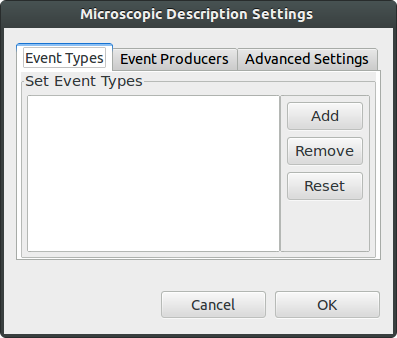
\includegraphics[scale=0.4]{images/state_settings.png}
	\caption{Aggregation Settings}
	\label{microSettings}
\end{figure}

In the aggregation settings, by default, all the event types and all the event producers are selected. The available settings are:
\begin{itemize}
	\item in the \textit{Event Types} tab, the filtering of the event types involved in the analysis;
	\item in the \textit{Event Producers} tab, the filtering of the event producers (the resources that produce the events) involved in the analysis. The producers are shown with their hierarchy, and depending on whether the operator required a valid hierarchy or not\footnote{The spatio-temporal operators take into account the hierarchy, while the temporal ones do not.}, the deselection of a parent node can lead to the deselection of its children nodes. The \textit{Add Result} button enables to load a set of event producers saved as an analysis result by another tool.
\end{itemize}

\subsubsection{Visualization Settings}
\label{visuop}
The \textit{Visualization} combo (\textcolor{red}{4} in Fig. \ref{traceConf}) provides a list of available views, in accordance with the compatibility of the previously selected metric and aggregation operator. The currently available choices are:
\begin{itemize}
	\item \textit{Partition}: is a visualization showing aggregates that correspond to an homogeneous behavior in the trace. The aggregates are separated by a blank space and all have a different colors. For a temporal aggregation, the available parameters in \textit{Settings} are:
	\begin{itemize}
		\item \textit{Aggregate parts}: gather time slices that belong to the same aggregate. If not active, each time slice is separated, and their aggregation is shown thanks to their color.
		\item \textit{Show part number}: display the number of each aggregate part to help distinguishing them.
	\end{itemize}
	\item \textit{Temporal Stacked Bar Chart}: is a visualization showing the same aggregates as in \textit{Parts}, but also the proportion of event occurrences (or the ratio of state duration, if state distribution was selected in the previous step) for each aggregate. In this visualization, each event/state is separated vertically in each aggregate and their proportion is shown by making the height of each event/state in an aggregate proportional to its occurrence/duration. The events/states that have a proportion too small to be visible, are aggregated and displayed on top of the aggregate as a dotted line. In the \textit{Settings} window, you can customize the color of each event.
	\item \textit{Mode}: is a visualization based on the value that appears most often\footnote{It is based on the notion of mode in statistics \url{http://en.wikipedia.org/wiki/Mode_(statistics)}}. It is available for both temporal and spatiotemporal aggregation operators. In the \textit{Settings} window, you can customize the color of each event. In the settings of the spatiotemporal mode, you can also perform a filtering of the displayed event types. The difference with the event type filtering in the aggregation settings is that the aggregation process is performed with all the types selected in the aggregation settings, but the visualization takes into account only the types not filtered in its settings. 
\end{itemize}

\subsection{Quality Curves}
Ocelotl displays curves representing the different aggregation levels, as shown in Fig. \ref{aggregCurves}. The X axis is the aggregation ratio from 1 (fully aggregated) to 0 (maximal level of disaggregation). %(pIC), and the Y axis is the %TODO what is it ?
The green curve shows the level of displayed complexity and the red is the level of displayed information. 
%These curves are tied since adding information, add more complexity and vice-versa\footnote{For more information, cf. \cite{}.}.
The vertical blue line shows the current value of the parameter.

\begin{figure}[h!]
	\centering
	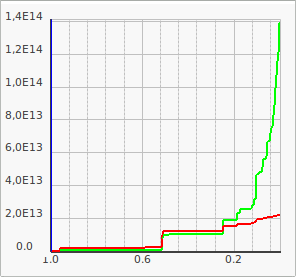
\includegraphics[scale=0.5]{images/ocelotlCurves.png}
	\caption{Quality curves in rising order.}
	\label{aggregCurves}
\end{figure}

\subsection{General Settings}
At the top right of the Ocelotl tool, a button (\textcolor{red}{1} in Fig. \ref{ocelotlButtons}) launches a window to configure the Ocelotl settings (Fig. \ref{ocelotlsettings}). When clicking \textit{OK}, the settings are saved for the current instance of Ocelotl. To permanently save the settings for all future instances of Ocelotl, click the button \textit{Save Settings}.

\begin{figure}[h!]
	\centering
	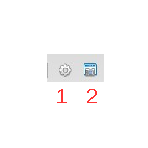
\includegraphics[scale=1.5]{images/ocelotlButtons.pdf}
	\caption{Ocelotl Features: 1. General settings; 2. Take a snapshot}
	\label{ocelotlButtons}
\end{figure}

\begin{figure}[h!]
	\centering
	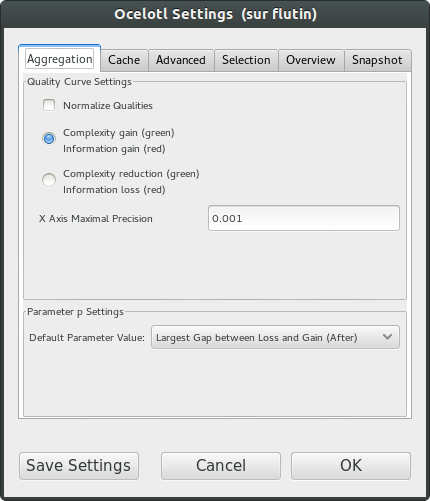
\includegraphics[scale=0.5]{images/ocelotlSettings.png}
	\caption{Ocelotl Settings}
	\label{ocelotlsettings}
\end{figure}

\subsubsection{Aggregation Settings}
The tab \textit{Aggregation Settings} contains two subsections: the \textit{Quality Curves} and \textit{Parameter P} settings. The \textit{Quality Curves} settings enables to change the appearance of complexity and information curves provided by the aggregation algorithm:
\begin{itemize}
	\item \textit{Normalize Qualities}: normalizes the curves and scale them on the interval $[0:1]$, which improves their readabilty. \underline{\textbf{Note:}} normalization should not be used with spatiotemporal operators since it provides incorrect results.
    \item You can choose between two representations of the curves: rising curves (complexity gain, information gain) or decreasing curves (complexity reduction, information loss).
    \item The \textit{Threshold} parameter determines the quality curves precision. The more its value decreases, the more the precision increases and the more aggregation steps are found. However, setting a too small value may lead to bad performances, so we advice to keep the default value.
\end{itemize}

The \textit{Parameter P} settings let you choose the strategy used to select the P parameter that will be chosen after launching an analysis.

\subsubsection{Cache Settings}
To prevent time-consuming loading of traces from the database, we use a cache system to accelerate access to the trace raw data. If the cache is enabled in the settings, then the first time a trace is analyzed, a cache file is generated. A cache file is a plain text file that contains non-null values of the trace, and each cache is specific to an metric operator, and a specific time region.

Several settings are available to configure the cache:
\begin{itemize}
	\item \textit{Cache Enabled}: allow to enable or disable the cache.
	\item \textit{Empty Cache}: delete all the cache files in the current cache directory.
	\item \textit{Datacache directory}: specify the directories where the cache files are stored.
	\item \textit{Maximum datacache size}: specify the maximum cache size in megabytes. When the maximum size is reached, the cache files with the oldest accessed dates are deleted until enough space is available. Specifying a value of -1 means that there is no maximal limit to the cache size.
	\item \textit{Cache time slice}: the first time a trace is loaded, a cache file is generated --- if the cache is enabled. This parameters specifies the number of time slices used for the generated cache. A higher number means a more accurate cache, but also a bigger cache file.
	\item \textit{Cache policy}: specify the rebuilding policy used to rebuild the data from the cache file when a "clean" rebuilding is not possible\footnote{A "clean" rebuild means that no time slice of the cache is split inside two time slices of the currently built microscopic description (such time slices are called "dirty" time slices). Typically it is clean when the number of time slices of the cache is dividable by the current number of slices (for example, if the cache was built with 10 000 time slices and the current rebuilt uses only 100 time slices, then one time slice of the new model will be built each from 10 time slices of the cache. But if the current rebuild is using 150 time slices, then some time slices of the cache would be split between two of the new time slices. The rebuild strategies are thus used for those "dirty" cases.}. The available choices are:
	\begin{itemize}
		\item \textit{Fast}: the dirty time slices are rebuilt by multiplying the values proportionally to the division of the cache time slice between the two new time slices (e.g. for a time slice which is split with 30\% of its time in one time slice and 70\% in the other, its values will be multiplied by 0.3 and 0.7 respectively). While this is a fast method, it may not be accurate in all cases (especially in cases with high ratio of dirty time slices).
		\item \textit{Accurate}: the dirty slices are rebuilt by performing a request to the database so that the events are rebuilt precisely. Depending on the event nature (punctual event, state, etc.), the rebuilding can be pretty slow.
		\item \textit{Automated}: try to automatically choose the best strategy between \textit{Fast} and \textit{Precise}. 
		\item \textit{Ask me}: show a dialog to the user at each run, from which he can select a strategy.
	\end{itemize}   
\end{itemize} 

If an aggregation was performed using an approximate strategy, a warning is displayed in the status bar of Eclipse.

\subsubsection{Advanced Settings}
In the \textit{Advanced Settings} tab, you can configure some advanced settings\footnote{\textbf{Note:} Modifying these values might decrease the trace reading performances.}:
\begin{itemize}
	\item \textit{Event Number Retrieved by Threads}: set how much events are loaded by threads for each iteration during the trace reading.
	\item \textit{Event Producers per Query}: enable to divide the query into several queries with a fixed number of event producers. This functionality is useful if the amount of free space on the drive is low, as the temp directory is used to store the query result during the trace reading. The default value is 0 which corresponds to fetching all producers in one query.
	\item \textit{Working Threads}: set the number of active threads during the trace reading. 
	\item \textit{Leave Aggregation}: it is possible to specify a maximum number of leaf event producers (i.e. event producers that have no child in the hierarchy). This is useful to bound the size and thus the memory footprint of the generated microscopic model, when there is a large number of event producers. If the maximum number of leaves is reached, then some event producers are aggregated at a hierarchical level. Ocelotl tries to find the node that will minimized the number of aggregated producers. This aggregation will of course affects the aggregation process, and thus displayed results might differ from the ones where no event producer is aggregated. If some event producers are aggregated, then a warning is displayed in the status bar of Eclipse. When performing a spatial zoom, if the number of leaves displayed is under the maximal bound, then the event producers are no longer aggregated.
\end{itemize}

\subsubsection{Snapshot Settings}
The \textit{Snapshot Settings} allow to set the saving directory of the snapshots taken in Ocelotl, as well as the resolution of the snapshot. The latter feature can be useful since drawing is relaunched by taking into account the new resolution, meaning that it can overcome the limitation of the screen resolution, and thus avoid any visual aggregations.

\subsubsection{Overview Settings}
The \textit{Overview Settings} allow to enable or disable the overview, along with customizing the color and transparency settings of the selection display on the overview.


\subsection{Time Settings}
In order to tune the time settings, several parameters can be modified in the bar under the graph display area (Fig. \ref{timeSettings}).
 
\begin{figure}[h!]
	\centering
	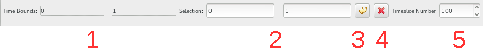
\includegraphics[width=1.0\textwidth]{images/ocelotl_bottom_time.pdf}
	\caption{Time Settings}
	\label{timeSettings}
\end{figure}

\subsubsection{Time Stamps}
There are two different time stamps values shown: the first one (\textcolor{red}{1} in Fig. \ref{timeSettings}) shows the starting and ending timestamps of the currently displayed zone of the trace, the second (\textcolor{red}{2}) shows the bounding time stamps of the currently selected zone (or are identical to the first ones, if there is currently no selection). The first time stamps are not editable, but the second sets of time stamps are, and allows to set the trace time bounds by modifying the values. The \textit{Cancel Selection} button  (\textcolor{red}{4}) cancels the current selection (both temporal and spatial) to the currently displayed time stamps and event producers. Alternatively, the selection can be canceled with a middle-click. The \textit{Reset} button (\textcolor{red}{3}) also cancels the current selection and in addition resets the temporal values to the global starting and ending time stamps values of the trace, and also resets the event producers to all the event producers present in the trace.

\subsubsection{Time Slices}
The \textit{Timeslice Number} field (\textcolor{red}{6}) corresponds to the number of time slices that will be used to compute the aggregation. It is advised to tune this parameter in order to find a granularity that is convenient to the analysis. As the aggregation algorithm complexity is dependent on this parameter, it is advised to increment it progressively to keep good performances.

\subsection{Analysis Settings}
To analyze the trace, several parameters allows to explore  different levels of aggregation and view. The aggregation settings are located under the \textit{Quality curves} display.
 
\begin{figure}[h!]
	\centering
	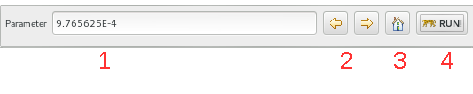
\includegraphics[scale=1.0]{images/aggregationSettings.pdf}
	\caption{Aggregation Settings}
	\label{aggregSettings}
\end{figure}

\subsubsection{Run an Analysis}
After having set the configuration, click on RUN! (\textcolor{red}{4} in Fig. \ref{aggregSettings}) (or press ENTER on the keyboard). The aggregation is then computed. This operation can take a while. When it is finished, the visualization and the curves are shown, as illustrated in Fig. \ref{showAggreg}.

\subsubsection{Change the Aggregation Strength}
In order to find a relevant aggregation, you can tune the \textit{Parameter} setting. This parameter allows to explore different aggregation levels, by navigating between different balances of the information loss and the gain in complexity. There are three ways to do this:
\begin{enumerate}
	\item Click on the curves. The corresponding parameter value is retrieved, and used to show the associated aggregation.
	\item Use the $<$- and -$>$ buttons (\textcolor{red}{2}) (or use left and right arrows on the keyboard). It increments or decrements the parameter.
	\item Enter a value manually, in the \textit{Parameter} field (\textcolor{red}{1}). The value must be between 1 and 0.
\end{enumerate}
A value of 1 means that the aggregation strength is maximal: all the trace is aggregated. On the opposite, a value of 0 means that each time slice is disaggregated. An intermediate value provides a compromise between both extrema. The button (\textcolor{red}{3}) resets the parameter to its default value --- i.e. the value displayed just after a run.

\subsubsection{Zoom}
Once you obtain an interesting aggregation level, you may want to focus on a particular time area. It is possible to zoom in on the trace by selecting an area by clicking and dragging with the left button of the mouse. Once the mouse is released the selection will adjust to the nearest selected time slice. It is is also possible to select just one time slice performing a simple click. Then, click on RUN! or press ENTER to display the selected area. In order to zoom out, you must click on \textit{Reset} and then on RUN!, to go back to the global view of the trace.

\paragraph{Spatial Selection}
If a spatio-temporal aggregation operator was chosen, then it is possible to perform a spatial zoom also. If more than one producer are selected, then the spatial selection automatically adjusts to the parent node containing all the selected producers. A click on the RUN! button will zoom on the selected area. A simple click selects a single producer, (or a single producer node, if a producer is too small to be represented), and a double-click selects the whole aggregate.

\paragraph{Zoom History}
During an exploration session of a trace, the zoom history is recorded, on both temporal and spatial dimensions (i.e. the selected time zones, and the selected event producers). It is possible to browse the history through the $<-$ and $->$ buttons in the bottom bar (cf. \textcolor{red}{5} in Fig. \ref{timeSettings}). The $<-$ button shows the previous zoom value, and the $->$ button shows the next zoom value. The history is lost when a different trace or a different aggregation operator is selected.

\subsubsection{Switch to Another View}
\begin{figure}[h!]
	\centering
	
\includegraphics[scale=1.0]{images/framesoc_buttons.png}
	\caption{Framesoc tools buttons}
	\label{framesocTools}
\end{figure}
It is possible to display the trace with the other visualization tools integrated in Framesoc: a Gantt chart, an event table, a statistics pie chart and a density chart. This is performed by clicking on the corresponding button in the top right corner, shown in Fig. \ref{framesocTools}. The newly opened view will show the events of the trace that are within the time bounds shown in the \textit{Start} and \textit{End} fields. You can focus on an area by selecting it with the mouse left button and then switching directly to another view, without loading the aggregation with the RUN! button. 

\subsection{Graph Display}
\begin{figure}[h!]
	\centering
	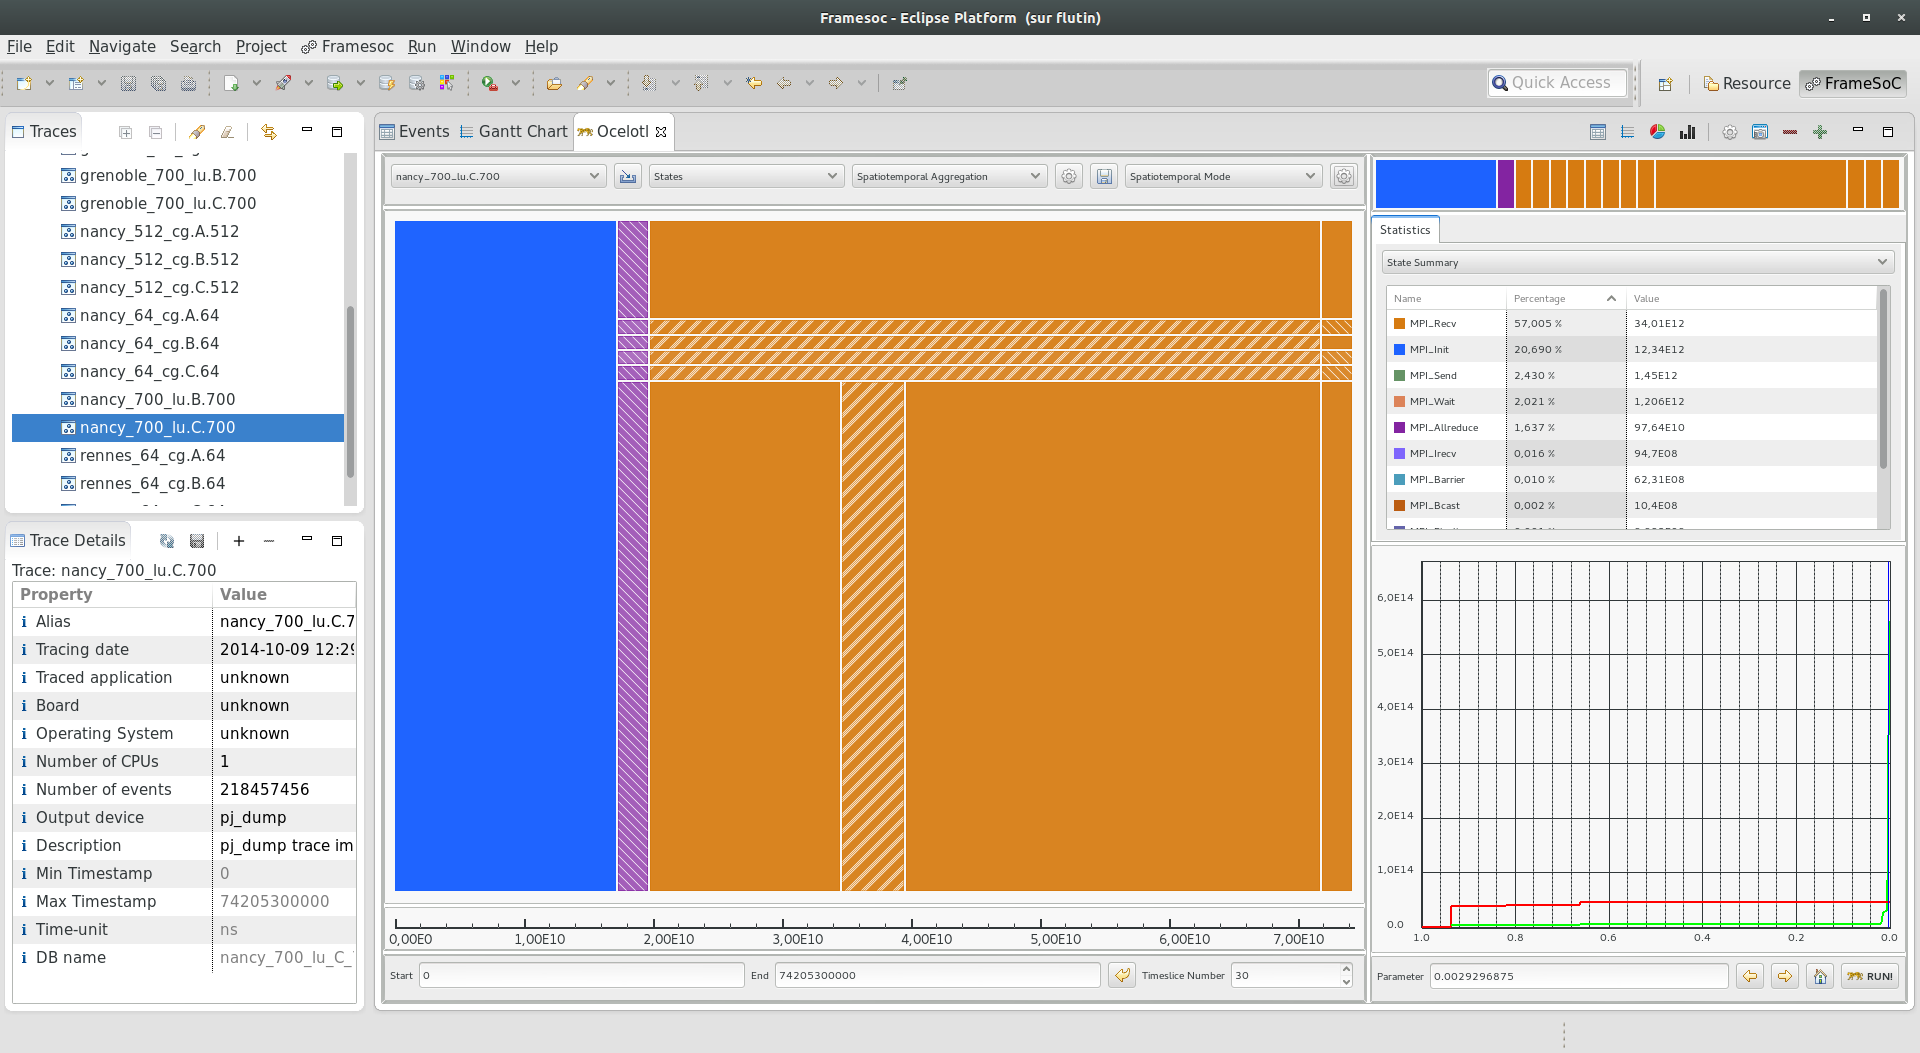
\includegraphics[width=1.0\textwidth]{images/ocelotlAggregated.png}
	\caption{A graph showing an aggregated trace}
	\label{showAggreg}
\end{figure}

Fig. \ref{showAggreg} shows an aggregated trace, with the proportion view. At the bottom of the graph, a time axis shows the time stamps of the currently displayed events. Events of different types have different colors. By letting the mouse over a part of the graph for a short time, a tooltip note shows the type of events represented by that part of the graph. For the event view, this note also displays the number of occurrences of the events divided by the duration of the aggregate\footnote{The time unit of the trace is displayed in the \textit{Trace Details} tab on the left bottom of the screen.}. For the state view, it is the state duration divided by the aggregate duration.

\subsubsection{Spatio-temporal Aggregate}
If a spatio-temporal aggregation is used, it is possible that the size of the window does not allow to correctly display the aggregates, especially if there is a great number of producers. If in the aggregate there is only disparities on the spatial level, then the aggregate is displayed with right to left stripes. If the disparities are also temporal, then the stripes go from left to right. Both of these cases can be seen in Fig. \ref{showAggreg}. In any case, to display the content of the aggregate, right-click on the aggregate and the content will be displayed in a new window. To close the newly created window, simply click on it.

\subsubsection{Y Axis}
Depending on the selected aggregation operator and visualization type, a Y axis displaying some additional information will appear on the left side of the graph display. For spatiotemporal aggregation, the Y axis displays the hierarchy of the event producers. This can be seen in Fig. \ref{showAggreg}. The hierarchy is shown as a set of rectangles, each representing a level of the hierarchy --- from left to right, the more general to the specific (typically root, cluster, machine, node). By hovering the mouse, the tooltip displays the name of the producer. If there is not enough place to correctly display the producers, they will be aggregated visually. By right-clicking on one of the producer, a hierarchy tree with the selected producer as root will be shown in a new window. Additionally it can be used to select the event producer for the whole displayed time region, by simply clicking on the producer.

In the case of a proportion view with a temporal aggregation, the Y axis displays the proportion value. When available, the unit is displayed at the top of the Y axis.

\subsection{Load and Save a Cache File}
\subsubsection{Load}
An alternative way to load a trace, instead of using the combo box, is to load it from its cache file, by using the button to the right of the combo box (element \textcolor{red}{5} in Fig. \ref{traceConf}). It opens a new window, allowing to select a cache file. If the selected cache file is valid and corresponds to a trace currently in the Framesoc database, then the trace is automatically loaded with the settings saved in the cache file.

\subsubsection{Save}
Once a run has been performed on a trace, a cache file is generated, in order to speed up the next analysis of the trace. It is then possible to save this cache to a specific location, in order to get a fast access later. This is done by pressing the button to the far right of the \textit{Aggregation Operator} combo box (element \textcolor{red}{6} in Fig. \ref{traceConf}).

\subsection{Overview}
\begin{figure}[h!]
	\centering
	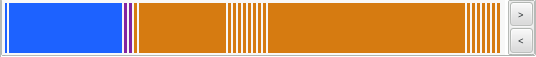
\includegraphics[width=0.7\textwidth]{images/overview.png}
	\caption{An overview of a trace}
	\label{overview}
\end{figure}
In the top right corner, Ocelotl displays an overview of the current trace, which gives the context of the trace. When a zoomed view of a trace is displayed, the overview highlights in red the currently displayed view. When selecting a part of the view on the graph, the corresponding selection is highlighted in blue on the overview.

The overview shows a temporal summary of the currently displayed trace. It is based on the mode operator described in subsection \ref{visuop}. The two small button on the right of the overview can be used to modified the aggregation level of the overview, and works in a similar fashion that the buttons \textcolor{red}{2} in Fig. \ref{aggregSettings}. Alternatively, you can also use the keys \textit{u} and \textit{i} to browse between aggregation levels.

\underline{\textbf{Note:}} Since the overview is computed in a different thread, there may be a delay between the display of the main graph and the apparition of the overview.

\subsection{Statistics}
\begin{figure}[h!]
	\centering
	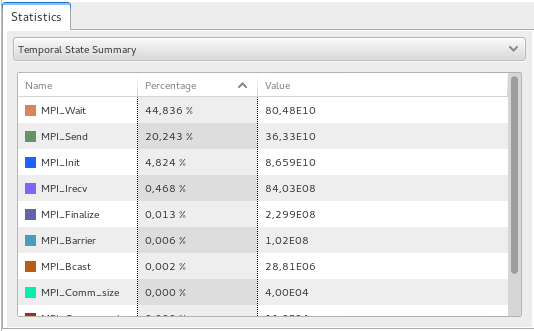
\includegraphics[width=0.7\textwidth]{images/statistics.png}
	\caption{An example of statistics}
	\label{stats}
\end{figure}
Ocelotl displays statistics about the currently selected data (as illustrated by Fig. \ref{stats}). The data selection is performed by dragging the mouse in the display of the aggregated graph, or, to select a single time slice, by performing a single click on the desired time slice. The statistics display is updated when the mouse button is released. To reset the selection, click on the \textit{Reset} button (\textcolor{red}{3} in Fig. \ref{timeSettings}) which sets the statistics data for the whole displayed region. 

The combo box lists all the compatible statistics operators for the currently selected operators. For now, only one statistic operator is available. It summarizes the data of the currently selected time region:
\begin{itemize} 
	\item If the \textit{Events} metric is selected, then all events are considered to be punctual events, then the statistics display shows for each type of events their number of occurrences.
	\item If the \textit{States} metric is selected, then the statistics display shows the portion of time spend in this state during the selected time region. Note that the total percentage can be different of 100\% since some event producers can be in no active state, leading to a total under 100\%. It is also possible possible to have more than 100\%, since some states can be embedded, meaning that an event producer can have more than one active state.
\end{itemize}

The statistics can be sorted by clicking on the column names of the table.

\subsection{Take a Snapshot}
In order to save the currently displayed diagram and curves, it is possible to save them as image files along with the current parameters of the trace in a text file. This is done by clicking the button at the top right of the display (\textcolor{red}{2} in Fig. \ref{ocelotlButtons}).

\subsection{Known Issues}
You may need to resize manually the different views, according to your resolution. Another problems is that the temporal selection between the main graph and the time axis view have a few pixels of difference.

For a list of all the current known issues in Ocelotl, please refer to the issues section of our github\footnote{\url{https://github.com/soctrace-inria/ocelotl/issues}}.

\newpage

%% bibliography
\newpage
\bibliographystyle{unsrt}
\bibliography{ocelotl_biblio}{}
%%

%%=====================================================================
%%=====================================================================
\end{sloppypar} 
\end{document}
%%=====================================================================
%%=====================================================================

\endinput
%%
%% End of file.
